\chapter{Аналитический обзор современного состояния исследований в предметной области}\label{ch:ch1}

\section{Определения рамок обзора}\label{sec:ch1/sec1}

\section{Предпосылки появления модульного оборудования}

\subsection{Многофункциональные универсальные металлорежущие станки}

Многофункциональные универсальные станки появились в начале 20 века и сочетали в себе различные функциональные возможности по обработке металлических заготовок. Все функциональные блоки размещались на одной станине и в зависимости от потребностей производства могли устанавливаться или сниматься, формируя различные конфигурации оборудования. Отличительной особенностью подобных станков была возможность работы на одном станке нескольких рабочих одновременно.

В качестве примеров подобного оборудования можно привести следующие многофункциональные универсальные станки:

\paragraph{Dalton Combinantion Machine}

Dalton Combinantion Machine или <<Комбинированный станок>> Далтона~(рисунок~\cref{fig:dalton}) представлял собой большой и тяжелый станок, основанный на стандартной станине и суппорте токарного станка Dalton; эта модель появилась в феврале 1923 года и была защищена многочисленными патентами. Станок первоначально позиционировался как <<представляющий особый интерес для владельцев гаражей и пароходов>> и, как утверждалось, занимал <<пятую часть площади, занимаемой отдельными станками того же типа>>. Несмотря на большое количество обрабатывающих модулей использовать все комбинации сразу на Далтоне было непрактично. Основой конструкции был 13-дюймовый токарно-винторезный станок, на который со стороны передней бабки крепились модули, реализующие функции горизонтально-фрезерного станка с приводным столом размером 24 x 7,5 дюйма, и комбинированного вертикально-фрезерного с пинолью для сверления. 

Самой оригинальной особенностью станка было устройство, с помощью которого мощность подавалась на вертикальные фрезерную и сверлильную головки. В сочетании с коническим шкивом передней бабки, задним редуктором и встроенной коробкой передач, это устройство могло дать фрезерной и сверлильной головке до восемнадцати скоростей. Верхняя часть опоры оправки для горизонтального фрезерного станка была сделана так, чтобы проходить через верхнюю часть передней бабки и, таким образом, в некоторой степени укрепляла конструкцию.

Токарный станок имел межцентровое расстояние равное 37 дюймов в версии со стандартной станиной и 73 дюйма при реализации на длинной станине. Причем последняя поддерживалась третьей опорой, расположенной между двумя внешними. Шпиндель с подшипником из фосфористой бронзы с конусом Морзе имел шесть скоростей, от 20 до 441 об/мин, проходное отверстие диаметром 11/16 дюйма. При этом вся эта <<модульная система>> работала от одного двигателя мощностью 1,5~л.\:с.

\begin{figure}[ht]
	\centerfloat{
		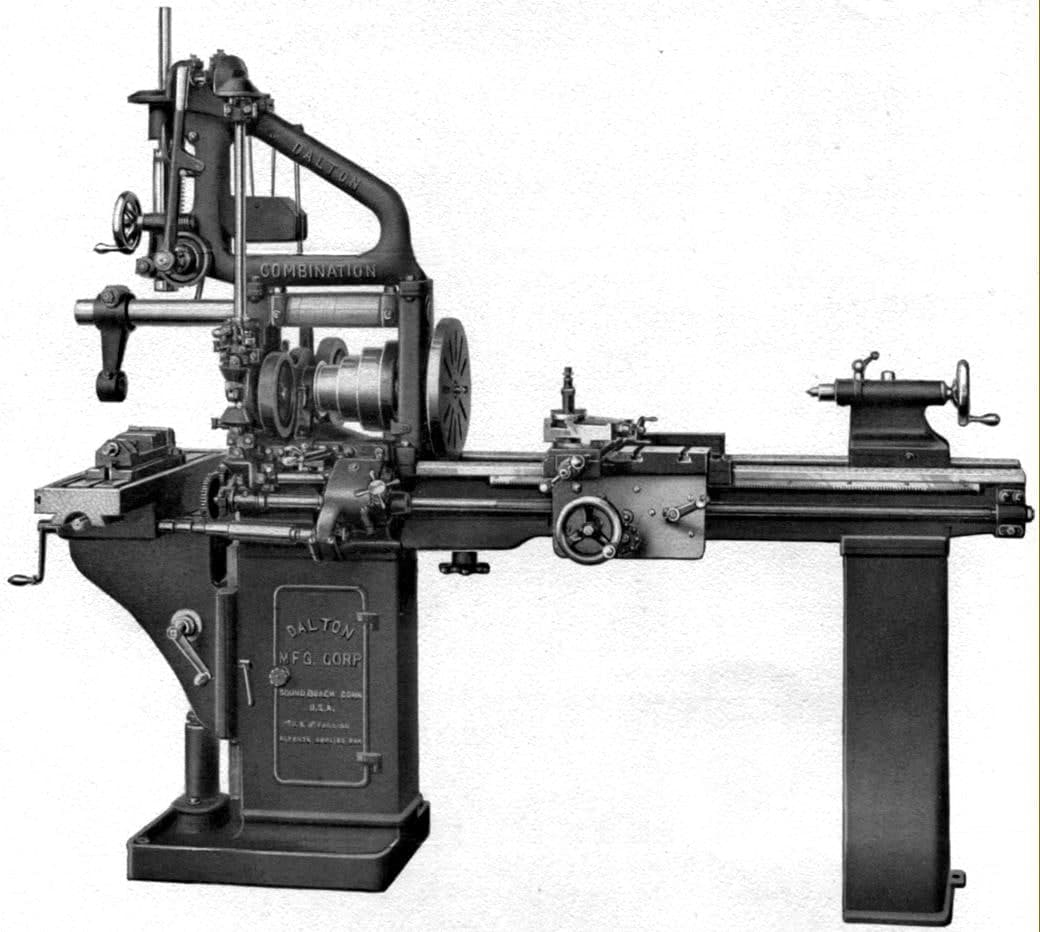
\includegraphics[width=0.7\textwidth]{ch-1/dalton}
	}
	\caption{Dalton Combinantion Machine.}\label{fig:dalton}
\end{figure}

\paragraph{Piho Combination Machine}

Piho Combination Machine~(рисунок~\cref{fig:piho}) "--- комбинированный универсальный станок, производимый в конце 1940-х годов компанией Hartensteiner Maschinenfabrik, рекламировался производителем как устройство, которое будет использоваться в ремонтных мастерских. Существовало два типоразмера: б\'ольшая версия имела возможность регулирования высоты заднего центра в диапазоне от 175 до 300\:мм и межцентровое расстояние равное 1300 мм; меньшая (настольная версия) "--- от 60 до 100\:мм и 180\:мм между центрами соответственно. Обе модификации могли работать как токарный станок, а также как горизонтальный и вертикальный фрезерный станок.

Несмотря на компромиссы, заложенные в конструкции, в станке были реализованы составные направляющие скольжения, низкоскоростной узел заднего редуктора, ходовой винт, движущийся под станиной, а также был оснащен барабаном для реверса шпинделя и тонкой подачей с ременным приводом. Очевидно, что в качестве токарного станка он работал так же, как и любой другой обычный токарный станок даже меньшего типоразмера. Однако наличие дополнительного фрезерного модуля, позволяло ему приблизится по своим возможностям к современным обрабатывающим центрам. Более того, фрезерный модуль был оснащен пинолью для быстрой подачей для сверления и имел возможность наклона в плоскости, перпендикулярной оси токарного станка. За счет большого размера расточного стола можно было ещё повысить универсальность станка, используя его в качестве горизонтального фрезерного.

\begin{figure}[ht]
	\centerfloat{
		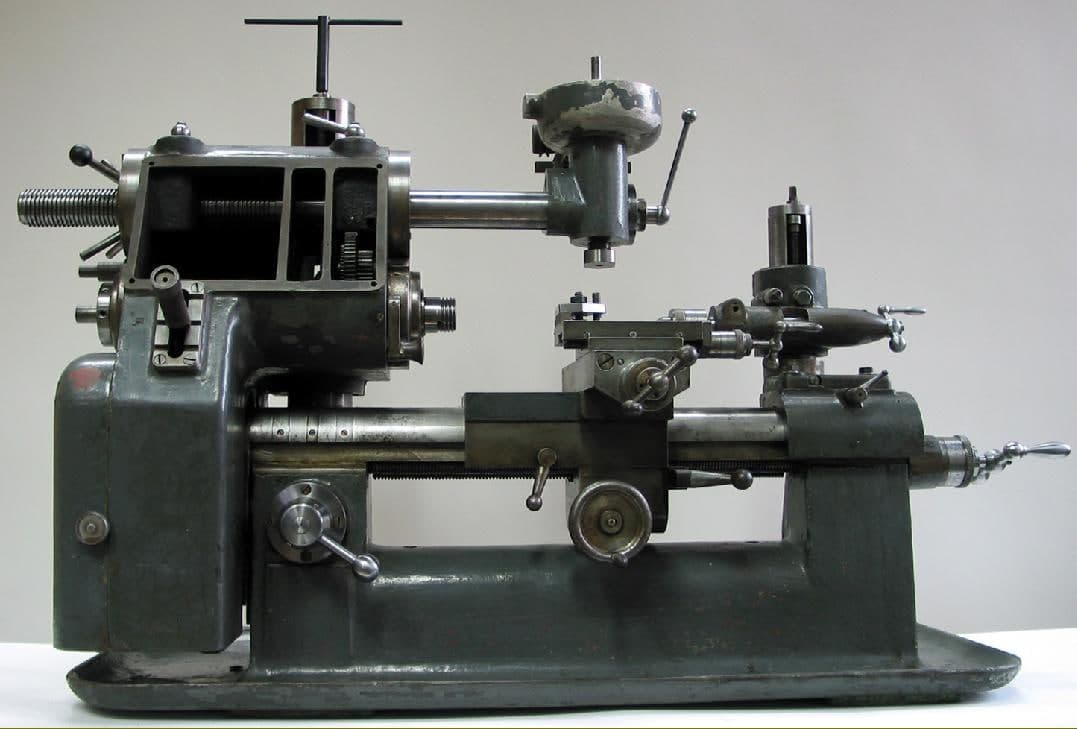
\includegraphics[width=0.7\textwidth]{ch-1/piho}
	}
	\caption{Piho Combination Machine.}\label{fig:piho}
\end{figure}

\paragraph{Adcock \& Shipley Combination Machine Tool}

<<Универсал>> Adcock \& Shipley~(рисунок~\cref{fig:adcock-1}) обладал максимальной гибкостью и модульностью по сравнению с другими подобными станками. На площади всего 7 футов на 3 фута для б\'ольшей модели и 11 футов 6 дюймов на 3 фута 8 дюймов для меньшей помещались токарно-винторезный станок, круглошлифовальный станок для внутреннего и внешнего шлифования, вертикальный/горизонтальный фрезерный станок, а также сверлильный станок и специализированные модуля для заточки инструмента. Вместо выдвижных или подъемных станин и передней бабки, которые использовались на многих других станках того же типа, Ryder был построен на основе обычного токарного станка, причем каждый отдельный модуль имел автономный привод и мог (кроме шлифовального станка) работать параллельно с другими модулями. Устройство было первоначально разработано для использования на борту корабля и соответствовало различным требованиям, установленным Британским адмиралтейством для этой цели. 

\begin{figure}[ht]
	\centerfloat{
		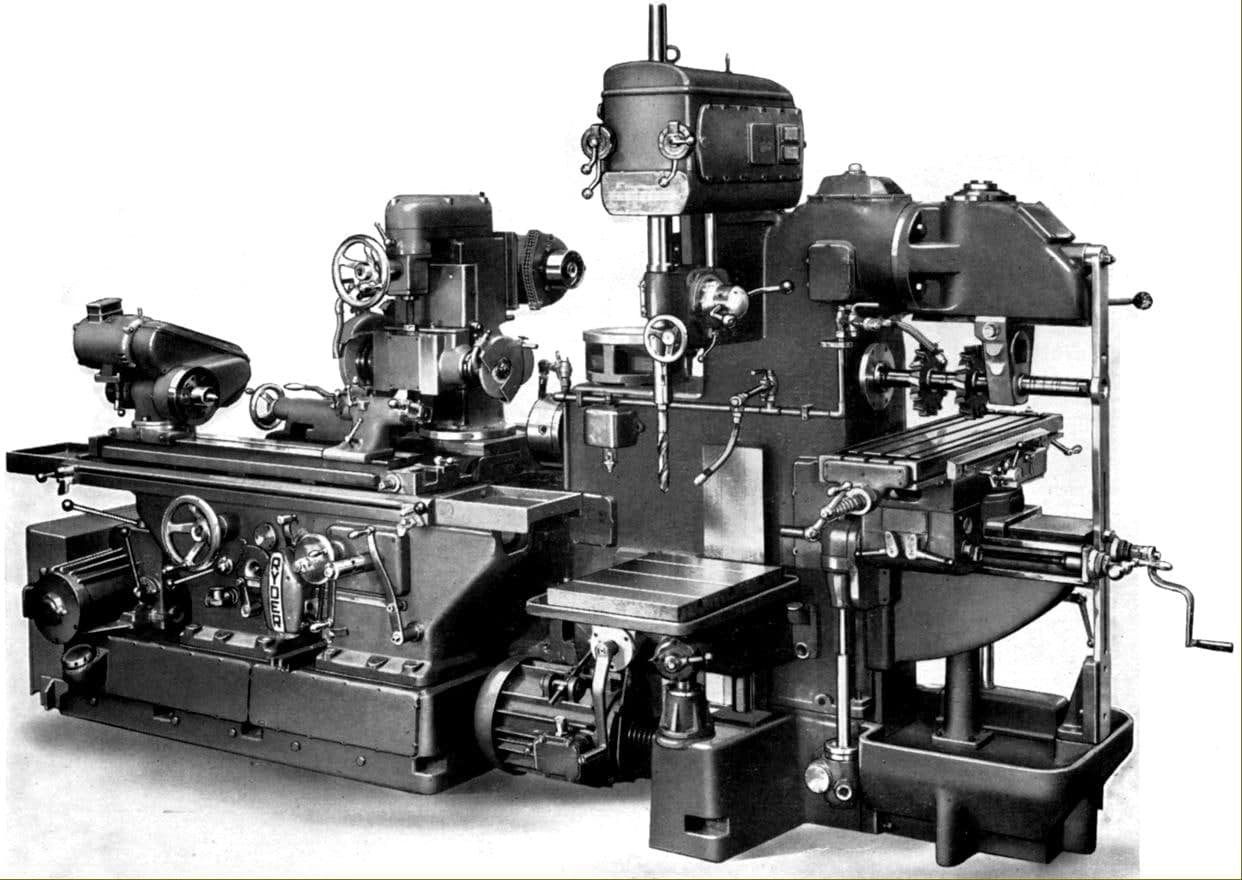
\includegraphics[width=0.7\textwidth]{ch-1/adcock-1}
	}
	\caption{Adcock \& Shipley Combination Machine Toolо, вид спереди.}\label{fig:adcock-1}
\end{figure}

Токарный модуль обладал следующими характеристиками: высота над станиной 8 дюймов, расстояние между центрами 18 дюймов, коробка передач из 8 скоростей, обеспечивающая максимальную частоту вращения шпинделя в 1020 об/мин., трехфазный привод на 3 л.с., 1760 об/мин. Проходное отверстие шпинделя было всего 0,75 дюйма, что вряд ли соответствовало той работе, для выполнения которой мог бы потребоваться рассматриваемый станок. Также на станке был установлен упрощенный редуктор для нарезания резьбы с ходовым винтом, позволявшим нарезать дюймовые резьбы с шагом от 4 до 100 ниток на дюйм. Для автоподачи суппорта использовался отдельный ходовой вал, а ходовой винт был нужен исключительно для нарезания резьб.

Фрезерный модуль обладал оригинальной конструкцией с горизонтальным и вертикальным шпинделями. Рабочая поверхность фрезерного стола была размером 26 на 6 дюймов с продольным ходом 10 дюймов и поперечным всего 5,5 дюйма, вертикальный ход стола составлял 10 дюймов, что было крайне мало по сравнению со схожими по размерам универсальными фрезерными станками того времени. Оба шпиндели были рассчитаны на инструмент под конус ISO 40, горизонтальный мог вращаться с частотой от 48 до 970 об/мин, вертикальный "--- от 77 до 1575 об/мин.

Универсальный стол шлифовального станка с возможностью поворота на 45 градусов по часовой стрелке и 15 градусов против часовой стрелки был установлен параллельно станине токарного станка и использовался как опора для шлифовальной головки. Два зубчатых колеса соединяли головку с органами управления в передней части станка. Максимальная высота заготовки над столом составлял 7 дюймов, максимальная длина "--- 10 дюймов. Также была возможна заточка различного режущего инструмента. Подача охлаждающей жидкости к шлифовальной головке представляла собой отдельный блок, разработанный, чтобы избежать загрязнения другой охлаждающей жидкости (подаваемой на токарный, фрезерный и сверлильный модули) абразивными частицами.

Сверлиьлный модуль устанавливался на задней части <<шпиндельной бабки>> токарного станка и имел шесть скоростей от 420 до 5000 об/мин с мощностью, обеспечиваемой отдельным двигателем мощностью 0,5 л.с. Диапазон выбора инструмента был обусловлен использованием в патроне конуса Морзе 1, что ограничивало применение данного модуля для легких работ~(рисунок~\cref{fig:adcock-2}).

\begin{figure}[ht]
	\centerfloat{
		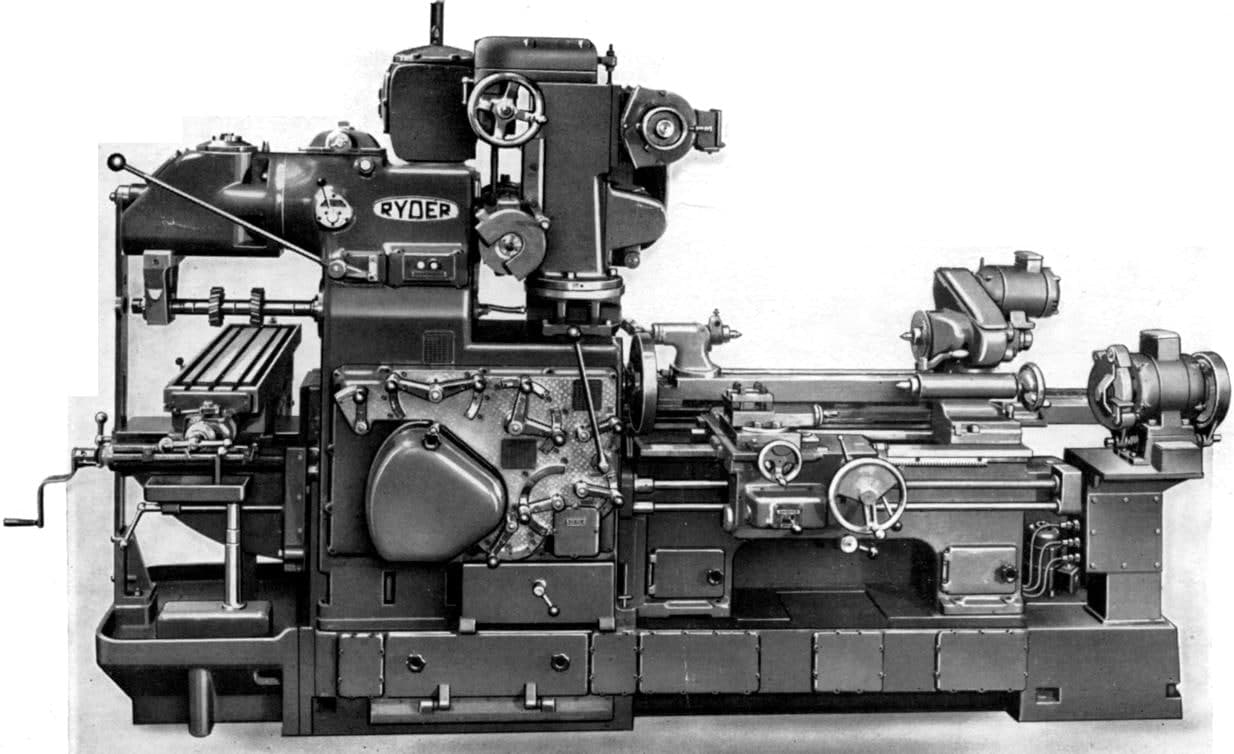
\includegraphics[width=0.7\textwidth]{ch-1/adcock-2}
	}
	\caption{Adcock \& Shipley Combination Machine Toolо, вид сзади.}\label{fig:adcock-2}
\end{figure}

\subsection{Агрегатные станки}

Агрегатными станками (АС) называется оборудование, которое состоит из стандартизованных и специальных агрегатов, сборочных узлов и деталей. Доля специально изготовленных узлом при этом меньше доли стандартизованных и нормализованных узлов. Конфигурация агрегатных станков происходит за счёт объединения всех его узлов в единый агрегат (станок, рабочий комплекс). Для данного агрегата всегда используется \textit{общая (монолитная)} системой управления и контроля. АС в подавляющем большинстве случаев применяют в \textit{крупносерийном и массовом производстве}. Первые агрегатные станки управлялись по аналогии со станками-автоматами, повсеместно распространенными в 60--70х годах, затем появились станки с ЧПУ. Это в свою очередь позволило использовать агрегатные станки уже и в серийном производстве. Все современные агрегатные станки управляются с помощью ЧПУ, однако в единичном и малосерийном производстве данный тип оборудования не использовался никогда. На агрегатных станках возможно осуществлять многоинструментную и многопозиционную лезвийную и абразивную механическую обработку деталей. Ранние представители агрегатных станков могли выполнять только один вид обработки (главным образом этим видом обработки было сверление и резьбонарезание). Существующие на текущий момент модели могут комбинировать практически все технологические операции по механической обработке.

Термин <<агрегатный станок>> впервые был использован и применялся в СССР. Однако существовали и существуют зарубежные станочные системы по сути своей являющиеся агрегатными станками. В литературе подобные станки именуются <<реконфигурируемыми производственными системами>>\footnote{От англ. \textit{Reconfigurable Machine Tools}.} или сокращенно RMS~\cite{lee1997reconfigurability, mehrabi2000}. RMS "--- это достаточно широкий класс промышленного оборудования, лишь некоторые разновидности которого соответствуют характеристикам отечественных агрегатных станков.  Так, в патенте~\cite{US6349237} описывается производственная система (станок), имеющая изменяемую структуру. Данная система разработана на основе рыночного спроса и может быть легко изменена для производства различных объемов продукции одного семейства. Описанная система включает в себя множество рабочих станций с реконфигурируемыми агрегатами, подсистему числового программного управления, включающую множество реконфигурируемых контроллеров, а также реконфигурируемую систему обработки материалов. Также в патенте показано, что предлагаемое аппаратное обеспечение позволяет преобразовывать станки, например, путем перемещения их шпиндельных узлов. Производственные мощности рассматриваемой системы быстро адаптируются к рыночным колебаниям спроса на продукцию. Функциональность легко адаптируется к производству новых продуктов того же семейства. Подобные станки облада.т определенными ключевыми характеристиками (например, модульностью, интегрируемостью, настройкой, конвертируемостью и диагностируемостью), которые необходимы для быстрой и рентабельной реконфигурации. Также в патенте предоставляется методика разработки таких станков и дополнительная методика для изменения производственной мощности, включая реконфигурацию и наращивание парка подобных станков. 

Существуют и другие подобные станочные системы, поэтому в рамках данного обзора под термином <<агрегатный станок>> будут, в частности, подразумеваться и зарубежные системы класса RMS. Как и любое другое оборудование приборостроительного производства, агрегатные станки делятся на специальными и специализированными. Очевидно, что специальные предназначены для обработки одной или несколько деталей одновременно, в свою очередь, специализированные агрегатные станки нацелены на последовательное формообразование нескольких деталей, требующего незначительного изменение конфигурации АС. В зависимости от потребностей производства АС могут работать как автономно, так и в составе гибких производственных систем.

Принцип агрегатирования АС базируется на том положении, что вместо проектирования всех узлов при создании нового станка используют ранее использованные узлы. Из данных узлов получается определенная компоновка, которая и становится новым станком. Для осуществления данного процесса заранее разрабатывается ряд однотипных узлов (агрегатов) разных типоразмеров и мощности приводов (если узел или агрегат включает в себя отдельную силовую часть). Узлы и агрегаты, входящие в этот ряд называются нормализованными или унифицированными. Нормализованные узлы дают возможность спроектировать АС, практически полностью удовлетворяющий используемому технологическому процессу обработки той или иной заготовки. Агрегатные специальные станки обладают рядом существенных преимуществ преимущества перед другими станками, применяемыми в массовом и крупносерийном производстве:

\begin{itemize}
	\item АС позволяют создавать станки специально под конкретный технологический процесс. То есть в случае применения АС у технологов появляется возможность сначала разработать телеологический процесс, а потом сконфигурировать под него АС из уже готовых и отлаженных узлов и агрегатов. При этом нет необходимости оптимизировать или изменять технологический процесс под конкретные производственные возможности.
	\item АС позволяют осуществлять многоинструментную обработку заготовок, что дает возможность существенно повысить производительность производства.
	\item АС дают возможность выполнения разнообразных технологических операций на одном и том же станке путем простое его переналадки.
	\item Использование АС позволяет непрерывно совершенствовать само оборудование, так как модернизируется не весь станок, а лишь тот узел (агрегат), который устарел. То же самое касается и ремонтопригодности, сломавшийся узел может быть быстро заменен на такой же работоспособный (находящий в резерве), а после ремонта основного первоначального узла, он будет возвращен на склад хранения, для резерва на случай будущих поломок.
	\item При использовании АС увеличивается надежность\footnote{Здесь под надежностью понимается способность оборудования сохранять в течение продолжительного промежутка времени значения своих основных параметров в заданных интервалах, а также выполнять все свои основные функции при заданных условиях применения. в установленных пределах значения всех параметров, характеризующих способность выполнять требуемые функции в заданных условиях применения.} работы оборудования, созданного из проверенных и отлаженных нормализованных узлов;
	\item В случае необходимости создания специального оборудования, оно также собирается из серийных узлов, что в целом удешевляет его.
\end{itemize}

Тем не менее, помимо плюсов, АС обладают и рядом недостатков, которые в настоящее время сильно сократили спрос на эти станки даже для \textit{массового производства}:

\begin{itemize}
	\item Для каждой новой выпускаемой на производстве детали, даже совсем незначильно отличающейся от уже существующей, необходимо делать (конфигурировать) новый специальный станок.
	\item АС в силу своей универсальности имеют более высоку стоимость, поэтому экономически могут оправдать себя только в условиях реального массового производства.
\end{itemize}

Для устранения этих противоречий надо, чтобы специальное станочное оборудование соответствовало трем главным условиям:

\begin{itemize}
	\item позволяло делать переналадку для обработки разных деталей при достаточно высокой производительности (это самое главное, потому что стоимость
	\item основных средств составляет значительную долю в себестоимости продукции);
	\item имело короткие сроки проектирования и изготовления;
	\item имело невысокую стоимость и быструю окупаемость.
\end{itemize}


Стоит отметить, что по большей части АС для \textit{отдельных производственных условий} могут удовлетворять всем этим требованиям. Рассмотрим более подробно принцип унификации, который применяется в АС, в дальнейшем это будет полезно для понимания отличий методики унификации АС и рассматриваемого в данной работе модульного технологического оборудования. Унифицированными (иначе нормализованными) узлами АС называются узлы, конструкции которых проектируются с той целью, чтобы быть основой для любого станка, который будет проектироваться на их основе. Из этого несложно сделать вывод о том, унифицированные узлы могут применяться в станках самых разных конфигураций. К нормализованных узлам АС относятся~(рисунок~\cref{fig:agr-machine}):

\begin{itemize}
	\item станины;
	\item поворотные делительные столы;
	\item силовые бабки;
	\item боковые станины;
	\item cтойки; 
	\item проставочные плиты.
\end{itemize}

\begin{figure}[ht]
	\centerfloat{
		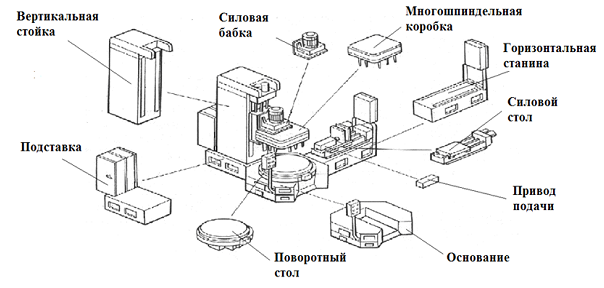
\includegraphics[width=\textwidth]{ch-1/agr-machine}
	}
	\caption{Структура узлов агрегатного станка.}\label{fig:agr-machine}
\end{figure}

В процессе многошпиндельной обработки массива отверстий или при фрезеровании плоскостей заготовок к силовым головкам крепятся специальные сверлильные и фрезерные насадки. В случае необходимости создания специальных узлов их компонуют из нормализованных сборок и деталей. Конструкция подобных узлов определяется в соответствии с конструкции детали, которая подлежит обработки на АС. Отечественные реализации АС включали в себя несколько сотен наименований различных унифицированных узлов в более, чем 2500 исполнений и типоразмеров. Из подобных нормализованных агрегатов и сборочных единиц могло состоять до 75--80\% узлов АС.

Необходимо отметить, что основное назначение АС "--- механическая обработка сложнопрофильных изделий. Из этого следует, что количество силовых узлов и инструментальных шпинделей, расположение осей шпинделей зависят от реализуемого на АС технологического процесса. Соответственно, по типу АС разделяются на: 

\begin{itemize}
	\item одноагрегатные;
	\item многоагрегатные;
	\item одношпиндельные;
	\item многошпиндельные;
	\item горизонтальные;
	\item вертикальные;
	\item наклонные;
	\item комбинированные;
	\item односторонние;
	\item многосторонние.
\end{itemize}

Очевидно,что однопозиционные АС в первую очередь рассчитаны на один неизменный установ заготовки. При этом обработка происходит с одной стороны, а положение заготовки в процессе обработки не изменяется. На многопозиционных станках, оснащенных поворотно-делительными столами механическая обработка заготовок может осуществляться в параллельном или последовательном режиме, но сразу в нескольких разных позициях относительно обрабатывающих инструментов.

Из всего вышесказанного можно сделать вывод о том, что основными нормализованными узлам АС являются так называемые силовые головки, определяющие технологическую операцию. В современных АС каждая силовая головка снабжена отдельным автономным электроприводом, поэтому могут сообщать какому-либо инструменту главное движение, либо осуществлять перемещение, например, делительного устройства. Для каждой силовой головки предусмотрен свой жестко запрограммированный цикл перемещения, включающий в себя подвод инструмента на ускоренной подаче, непосредственно рабочий ход инструмента (их может быть несколько в зависимости от технологического процесса), при необходимости может быть реализована выдержка в жёстком упоре и отвод инструмента на ускоренной подаче с последующем остановом. Как уже отмечалось ранее, первые образцы АС реализовывали данную циклограмму механически с помощью вращающегося кулачка, современные образцы АС реализуются ее исключительно посредством ЧПУ.

Параметры каждой силовой головки являются основанием для использования ее для конкретной технологической операции. К основным параметрами силовых головок относят:

\begin{itemize}
	\item мощность привода главного движения;
	\item наибольшая сила подачи;
	\item частота вращения приводного вала шпинделя головки;
	\item пределы перемещения при подаче;
	\item скорость холостого хода;
	\item скорость рабочего хода;
	\item длина рабочего хода;
	\item габаритные размеры.
\end{itemize}

Необходимо отметить, что силовые головки являются не единственными блоками АС. Для выполнения силовых операций: фрезерования с большим съёмом материала, растачивания, подрезки торцов большого диаметра требуются блоки большей жесткости. Для повышения жесткости силовых головок разработчики данной концепции пришли к следующему решению: агрегат, обеспечивающий главное движение отделили от механизма подачи силовой головки. Таким образом, получилось два разных независимых узла: отдельный силовой стол для подачи и силовая бабка для реализации главного движения.  

Помимо блоков, обеспечивающих прямолинейное движение заготовки по отношению к инструменту в АС часто применялись поворотные делительные столы, основной задачей которых было закрепление на них специализированных приспособлений с заготовками для их поворота на определенный угол. Данные столы имели возможность перемещать обрабатываемые заготовки из одной рабочей позиции (установа) в другую. При этом осуществлялось точное фиксирование заготовки относительно режущего инструмента. Поворотные столы могли быть в вертикальном или горизонтальном исполнениях. Форма столов чаще всего была либо кольцевая, либо дискообразная. Такие столы перемещались только в горизонтальной плоскости. Если поворотный стол осуществлял вращение в вертикальной плоскости, то такой блок именовался <<барабан>>. При использовании барабанных блоков, приспособления с закрепленными в нем заготовками располагалось на периферийной поверхности барабана и заготовку можно было обрабатывать с двух сторон одновременно.

К современным станкам, которые могут быть отнесены к классу агрегатных, можно отнести Mikron MultiX\footnote{\url{https://www.mikron.com/machining-solutions/machining-systems/highly-productive-systems/multix/}}~(рисунок~\cref{fig:mikron}). Данное оборудование представляет собой платформу, в которую могут быть установлены различные станции обработки. Платформа выступает в качестве базового агрегата, а обрабатывающие станции являются сменными блоками. Существует три типоразмера базового агрегата, различающиеся количеством устанавливаемых на них блоков. Конфигурация платформы подбирается под конкретный технологический процесс.

\begin{figure}[ht]
	\centerfloat{
		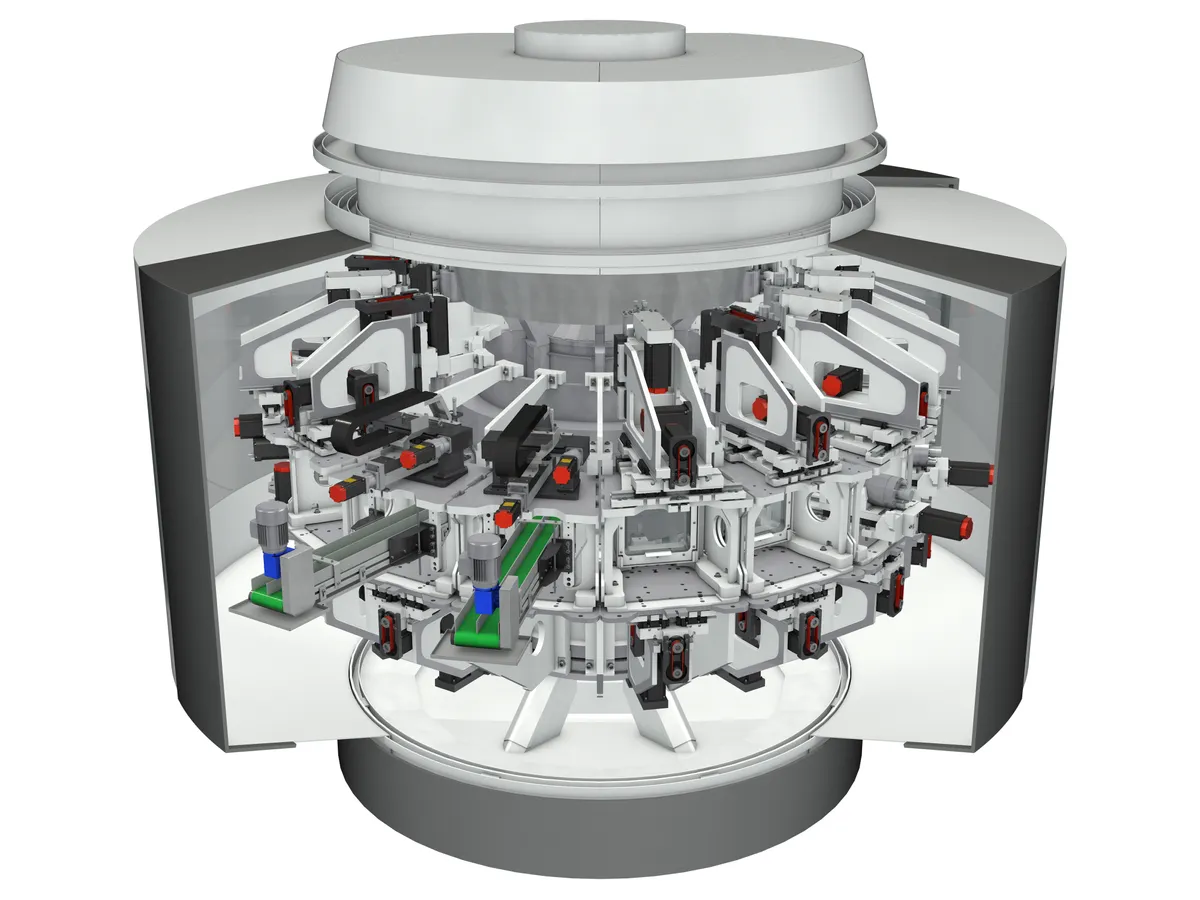
\includegraphics[width=0.7\textwidth]{ch-1/mikron}
	}
	\caption{Агрегатный станок Mikron MultiX.}\label{fig:mikron}
\end{figure}

Таким образом, можно прийти к выводу, что унификация и стандартизация АС сильно усложняется, т.\,к. конструкция не может быть разделена на равные по своим возможностям и габаритам блоки. По сути АС "--- это сложный унифицированный станок-автомат, где каждый блок имеет несколько разных исполнений, что в общем дает большое разнообразие полученного таким образом оборудования, но это оборудование нельзя считать модульным. Блоки АС неуниверсальны и могут выполнять свои функции только вместе с другими блоками, проектирование которых происходило одновременно. Агрегатные станки унифицированы только по присоединительным размерам и нет центрального блока, на который могли бы устанавливаться другие блоки, изменяя тем самым основную функцию оборудования. Также стоит еще раз повторить, что в основном АС применялись только для металлообработки и никогда не использовались для других видов обработки. На сегодняшний день в силу своей сложности и узкой направленности АС потеряли актуальность даже в рамках массового производства, однако сами базовые подходы, которые были положены в основу их функционирования могут и должны быть использованы для создания универсального модульного оборудования для условий мелкосерийного и единичного производства. 

\section{Модульные системы управления технологическим оборудованием}\label{sec:ch1/sec2}

Анализируя развитие современной промышленности, можно прийти к выводу о том, что на сегодняшний день наиболее перспективным направлением развития в этой области является создание гибких распределенных автоматизированных производственных линий. Четвертая промышленная революция и постепенное внедрение кибер-физических производственных систем по-новому определяют само понятие массового производства.

Происходит последовательный переход от <<жестких>> конвейерных решений к малым партиям, выполняемым по индивидуальным заказам. Также не останавливается развитие  концепции малых инновационных предприятий и стартапов. Все это приводит к изменению подхода к проектированию современного интеллектуального оборудования. 

Первые станки с ЧПУ появились еще в 50-х годах прошлого века, и с тех пор их развитие не прекращается. Тем не менее, вектор этого развития всегда был ориентирован исключительно на массовое производство. Системы с ЧПУ всегда были и остаются сложными, высокопроизводительными, а самое главное "--- очень дорогим. Процесс внедрения подобных систем очень долог, а время жизни современных автоматизированных производств может исчисляться десятилетиями.

Конечно, все это усложняет внедрение современных коммуникационных технологий. Любое изменение требует либо полного перестроения устоявшейся производственной системы, либо создания дополнительного слоя управления, который позволит связать устаревшее оборудование с современной кибер-физической системой.

Такой подход представляется наиболее целесообразным в переходный период, но в дальнейшем от него, безусловно, придется отказаться. Необходим пересмотр самой парадигмы проектирования оборудования с ЧПУ. Нужно рассматривать любое новое оборудование с точки зрения возможности включения его в единую информационно-телекоммуникационную среду с использование открытого протокола.

Попытки реализации подобного подхода делались уже неоднократно. Например, в работе Grigoriev and Martinov предлагается подход к построению переносимого ядра ЧПУ на основе платформы независимых библиотек. Открытая архитектура данной системы ЧПУ включает в себя уровни абстракции для реализации различных человеко-машинных интерфейсов, а также имеет возможность описания компонентов системы на различных языках программирования. Компоненты системы связываются между собой по шине Fieldbus [grigoriev2014research].

Bin et al. описывают открытую платформу для создания систем ЧПУ. Данная система состоит из набора универсальных компонентов, которые могут быть использованы повторно, а также коммуникационных модулей для их связи [bin2004research].

Morales-Velazquez et al. предлагают платформу с открытой архитектурой на основе многоагентной системы программно-аппаратных компонентов, именуемой MADCON. The Аппаратные блоки предлагаемой системы объединяют функции управления и мониторинга, обеспечивая открытую архитектуру на базе FPGA для реконфигурируемых приложений. Компоненты программного обеспечения используют структуру XML для файлов описания системы, собирая такие функции, как язык описания блок-схем и графический интерфейс пользователя [morales2010open] 

В работах Verba et. al[verba2017platform] и  Prazeres and Serrano [prazeres2016soft] рассматривается очень интересная концепция Fog of Things. Данная концепция является развитие концепции Internet of Things, являющейся основой многих кибер-физических производственных систем. Fog of Things позволяет создать более однородную информационно-телекоммуникационную среду за счет совершенствования и упрощения протокола взаимодействия компонентов.

В работе [morales2010open] представлена система ЧПУ с открытой архитектурой, основанная на авторской мультиагентной аппаратно-программной платформе Multi-Agent Distributed CONtroller (MADCON). Эта система имеет возможность реконфигурируемости и адаптивности. При проектировании интеллектуальных приводов для этой системы были использован структурированный подход к созданию программных и аппаратных составляющих. Аппаратные блоки предлагаемой системы объединяют в себе функции управления и мониторинга, обеспечивая открытую архитектуру на основе ПЛИС для обеспечения реконфигурируемости. С другой стороны, программные компоненты разработаны с использованием языка XML для описания системы, что позволило отказаться от привычного программирования и создавать логику программных компонентов с помощью визуальных блок-схем. MADCON был применен в качестве системы управления модернизированным токарным станком с ЧПУ для управления и контроля с целью проверки предлагаемой архитектура, которая может быть применена для создания интеллектуального производства нового поколения системы.

В [han2007development] рассматривается контроллер с открытой архитектурой, который может стать основой для различного оборудования с ЧПУ. Разрабатываемый контроллер имеет модульную арихтектуру, а в качестве аппаратной платформы использует персональный компьютер. Основная цель работы "--- разработать методику построения программно-аппаратная платформа системы ЧПУ. Также исследуются методы статического моделирования контроллера с открытой архитектурой, включающие технологию объектно-ориентированного программирования, технологию применения динамических библиотеки и разделения системных модулей. Авторы обсуждают динамическое моделирование поведения и представление потока данных контроллера с открытой архитектурой, которые описаны с помощью иерархической модели конечного автомата. Для разработки библиотеки программных функциональных компонентов авторы создали модель многократно используемого программного модуля. В качестве испытательного стенд выступает 3-осевой фрезерный станок. Для данного станка был успешно разработан программный код системы ЧПУ, основанной на описанной библиотеке функциональных модулей с применением методики конфигурирования системы. Результаты экспериментов показывали, что, помимо увеличения степени повторного использования программного кода и открытости, применение вышеупомянутой методологии приводит к значительному сокращению времени разработки, а также стоимости обслуживания конечного оборудования с ЧПУ.

\section{Промышленные аналоги предлагаемой модульной платформы}

Прямых аналогов предлагаемой концепции адаптивной платформы технологического оборудования авторами найдено не было, поэтому будут рассмотрены проекты и готовые продукты, сходные с МТП по тем или иным параметрам, первым из которых является \textit{универсальность рабочего органа}, то есть возможность путём простой переналадки менять тип оборудования. 

На сегодняшний день на рынке представлены несколько типов универсальных модульных настольных станков нижнего ценового диапазона. Одним из наиболее известных производителей подобного оборудования является компания \textit{Proxxon}~(рисунок~\cref{fig:proxxon}), выпускающая различные настольные станки <<хоббийного>> класса, в основном токарно-фрезерно-сверлильной группы, распиловочное оборудование и ручной электроинструмент. Большое количество универсальной оснастки и~взаимозаменяемость многих частей оборудования Proxxon позволяет использовать его в небольших мастерских, а также на малых инновационных предприятиях, но с рядом ограничений:

\begin{itemize}
	\item В базовой комплектации все оборудование ручное. Возможность переделки под числовое программное управление (ЧПУ) является опцией. Возможности ЧПУ сильно ограничены.
	
	\item Спецификации оборудования закрыты, создание своих модулей невозможно, либо возможно, но только с~применением реверс-инжиниринга.
	
	\item Как уже было отмечено выше, все оборудование Proxxon субстрактивного типа, возможность использовать его для создания 3d-принтера или контрольно-измерительной машины отсутствуют, так как нет единой модульной структуры блока управления ЧПУ, а также фирменного программного обеспечения.	
\end{itemize}

\begin{figure}[ht]
	\centerfloat{
		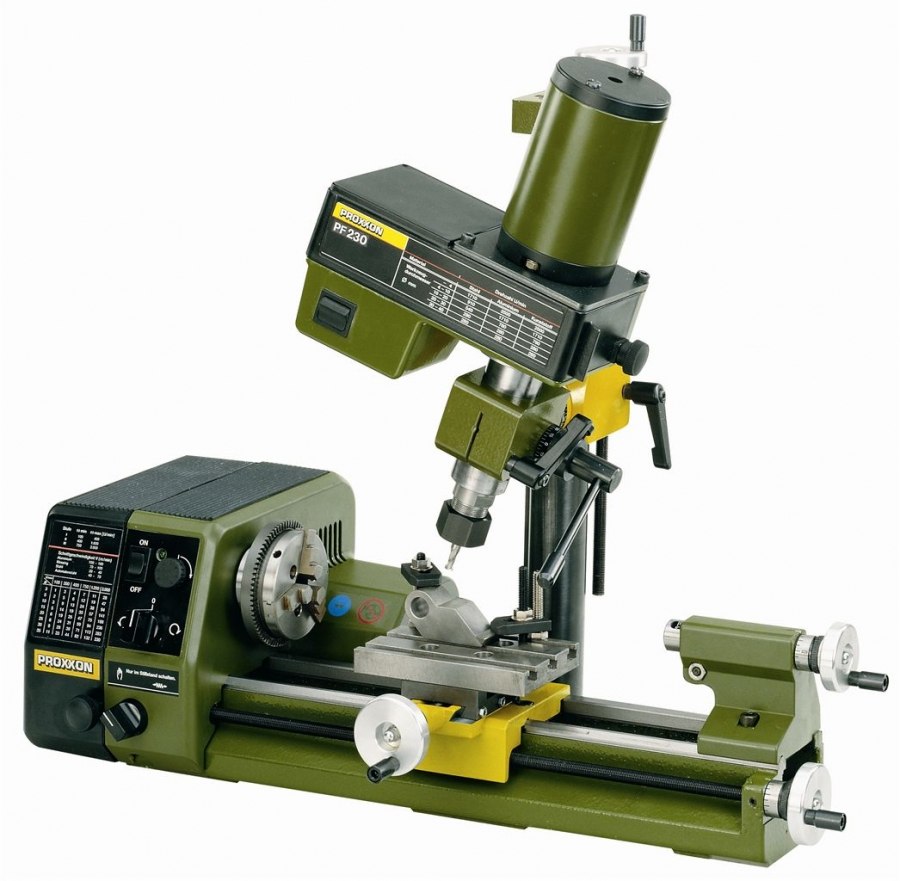
\includegraphics[scale=0.27]{ch-2/image1.png}
	}
	\caption{Пример оборудования компании Proxxon.}\label{fig:proxxon}
\end{figure}

Стоит также отметить настольные модульные универсальные станки, выпускаемый немецкой компанией TheCoolTool (thecooltool.com), в~особенности модели UNIMAT~1~(рисунок~\cref{fig:unimat-2}) и UNIMAT CNC~(рисунок~\cref{fig:unimat-2}).

\begin{figure}[ht]
	\centerfloat{
		\hfill
		\subcaptionbox{\label{fig:unimat-1}}{%
			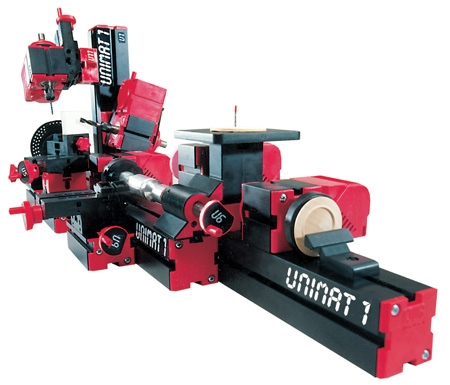
\includegraphics[width=0.4\linewidth]{ch-2/image2}}
		\hfill
		\subcaptionbox{\label{fig:unimat-2}}{%
			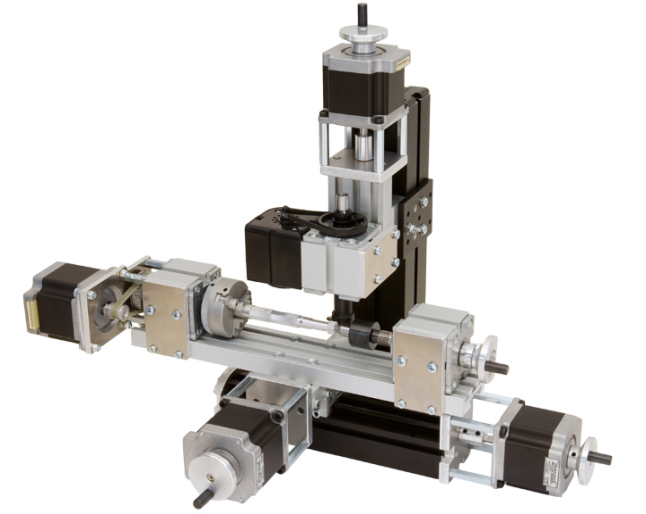
\includegraphics[width=0.4\linewidth]{ch-2/image3}}
		\hfill
	}
	\caption{Настольные модульные станки UNIMAT 1 (\textit{а}) и UNIMAT CNC (б).}\label{fig:unimat}
\end{figure}

Первый из рассматриваемых станков представляет собой модульную систему <<6 в 1>> с ручным управлением (переделка под ЧПУ возможна только с применением специальных доработок и реверс-инжиниринга), то есть позволяет в зависимости от компоновки модулей производить:
\begin{itemize}
	\item Распиловку деревянных и металлических заготовок вертикально расположенным ножовочным полотном.
	
	\item Токарную обработку деревянных заготовок.
	
	\item Токарную обработку металлических заготовок.
	
	\item Плоское торцевое шлифование с возможностью снятия шлифовального блока для ручной обработки шлифовальным кругом.
	
	\item Вертикальное и горизонтальное фрезерование.
	
	\item Сверление с возможностью поворота сверлильной головки на 360$^{\circ}$ или снятия её для ручного сверления.
	
	
\end{itemize}
Возможность совмещения двух операций без переналадки оборудования отсутствует.

Второй является токарно-фрезерно-сверлильным модульным станком с ЧПУ, в котором в зависимости от компоновки существует возможность управления шестью осями одновременно, что позволяет совмещать операции обработки без перенастройки модулей. Достоинством данного оборудования является большая открытость программной архитектуры, что подтверждается возможностью использовать для управления осями станка не только фирменное закрытое программное обеспечения, но и открытое решение EMC2, построенное на базе свободной операционной системы Linux. При этом сам станок представляет собой лишь набор управляемых электроприводов без внутреннего блока управления, что требует постоянного подключения к персональному компьютеру, приобретаемому отдельно.

К недостаткам можно отнести:
\begin{itemize}
	\item закрытую аппаратную архитектуру рассматриваемого продукта, что существенно усложнит переделку данного решение подо что-то отличное от металлообрабатывающих станков;
	
	\item неудачную геометрическую компоновку станка, что также ставит по сомнение возможность его переделки под другие нужды (например, очевидно, что подобная кинематическая схема вряд ли позволит использовать ее в качестве трёхмерного принтера или контрольно-измерительной машины);
	
	\item отсутствие портала, что влечет за собой снижение жёсткости связки координатных осей, а, следовательно, и жесткости станка в целом. Последнее будет особенно заметно при максимально удалении осей, из-за чего может пострадать точность обработки. Данное предположение подтверждается спецификациями, размещенными на сайте производителя, где указывается, что точность установки не может превысить 80мкм.
	
	\item низкую мощность приводов осей, а также очень небольшие рабочие ходы по некоторым из них.
	
	
\end{itemize}
Из всего вышесказанного можно сделать вывод о том, что за исключением возможности использования свободного программного обеспечения рассматриваемый продукт не удовлетворяет требованиям концепции МТП и не может быть рассмотрен в качестве её прямого аналога.

Второй параметр, по которому проводилось сравнение предлагаемой концепции с существующими аналогами "--- \textit{открытая аппаратная архитектура}, позволяющая создавать новые типы оборудования без необходимости создания каких-то дополнительных переходных блоков и применения реверс-инжиниринга.

Для сравнения были рассмотрены два проекта, целью которых является создание открытой платформы универсального оборудования с ЧПУ:

\begin{enumerate}
	\item \foreignlanguage{english}{\textbf{Build Your Own CNC}} (\href{https://www.buildyourcnc.com/cnckit2.aspx}{\foreignlanguage{english}{buildyourcnc.com}}).
	
	\item \textbf{Shapeoko} (shapeoko.com).
\end{enumerate}

Рассмотрим оба этих проекта более подробно. \textit{Build Your Own CNC}~(рисунок~\cref{fig:byocnc}) "--- коммерческий проект по созданию универсального сборного оборудования с числовым программным управлением. Может считаться условно открытым, так как с одной стороны на сайте производителя отсутствуют чертежи и прочая техническая документация, необходимая для самостоятельного изготовления того или модуля оборудования (за исключением файлов раскроя основных корпусных деталей), но с другой стороны компания принимает запросы от пользователей на создание новых модулей (новых типов оборудования). Финансирование данных исследований проводится за счёт средств, полученных в качестве пожертвований от пользователей, а также за счет основного бизнеса компании "--- производства и продажи модулей и готовых сборных устройств.

На сегодняшний день в рамках проекта \textit{Build Your Own CNC} реализовано достаточно большое количество модулей и готовых устройств среди которых можно выделить:

\begin{itemize}
	\item Установку для лазерной резки и гравирования.
	
	\item Трёхкоординатное фрезерные и сверлильные станки различных компоновок и типоразмеров с множеством сменных головок, среди которых необходимо выделить печатающую головку, позволяющую создать на основе предлагаемой платформы 3d-принтер типа FDM\footnote{сокр.~от~англ. \textit{Fused Deposition Modeling} "--- моделирование методом наплавления.}.
\end{itemize}

\begin{figure}[ht]
	\centerfloat{
		\hfill
		\subcaptionbox{\label{fig:byocnc-1}}{%
			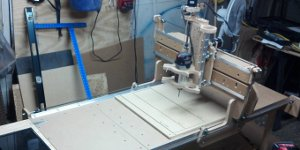
\includegraphics[width=0.5\linewidth]{ch-2/image4}}
		\hfill
		\subcaptionbox{\label{fig:byocnc-2}}{%
			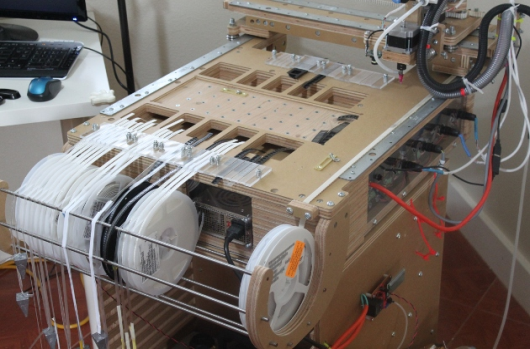
\includegraphics[width=0.5\linewidth]{ch-2/image5}}
		\hfill
	}
	\caption[Примеры оборудования, созданного в рамках проекта \textit{Build Your Own CNC}]%
	{Примеры оборудования, созданного в рамках проекта \textit{Build Your Own CNC}: фрезерный станок портального типа (\textit{а}), установка для позиционирования электронных компонентов на печатной плате (\textit{б}).}\label{fig:byocnc}
\end{figure}


\begin{itemize}
	\item Распиловочные вертикальные станки.
	
	\item Установку для автоматического размещения электронных компонентов на печатной плате (англ. \textit{Pick and Place machine}).
	
	
\end{itemize}
В планах компании также разработать:
\begin{itemize}
	\item Пятикоординатный фрезерный станок.
	
	\item 3d-принтер, использующий технологию фотолитографии.
	
	\item 3d-принтер, использующий технологию селективного лазерного спекания.
	
	\item Станки токарной группы.
	
	\item 3d-сканер.
	
	
\end{itemize}
К недостаткам данного проекта можно отнести следующие:
\begin{itemize}
	\item Как уже отмечалось ранее, проект не является полностью открытым с точки зрения аппаратного обеспечения.
	
	\item На текущий момент реализовано очень малое количество типов оборудования. Отчасти это связано с первым недостатком, так как спецификации закрыты и разработкой новых модулей и типов оборудования занимаются только сотрудники компании.
	
	\item Отсутствует единая универсальная кинематическая схема, из-за чего для каждого нового вида оборудования необходимо проектирование новой кинематической схемы, а также сопутствующие этому процессу расчеты и моделирование.
	
	\item Отсутствует единый подход к проектированию линейных приводов. Предполагается возможность использования как ходовых винтов с трапециевидной резьбой, так и передач на основе зубчатых ремней и цепей. Особо настораживает использование цепных передач в прецизионных настольных станках для установки электронных компонентов на плату.
	
	\item Основной материал, из которого изготавливаются все несущие и корпусные детали всех видов оборудования "--- клеевая фанера. При всех очевидных достоинствах данного материала таких, как легкость обработки, хорошее виброгашение, высокая прочность, низкая цена, целесообразность использования данного материала для создания высокоточного оборудования с ЧПУ вызывает большие сомнения. Очевидно, что авторам проекта вряд ли удалось достичь высокой жесткости конструкции и точность оборудования оставляет желать лучшего.
	
	\item Привода всех модулей и всех типов готового оборудования не имеют никаких датчиков обратной связи по положению. Авторы проекта исходят из предположения, что используемые ими шаговые двигатели никогда не пропускаю шагов, драйверы шаговых двигателей всегда генерируют правильную последовательность импульсов, а используемые кинематические схемы не подвержены заклиниванию.
	
	\item Компания не занимается производством или разработкой блоков управления для своего оборудования и вообще каких-либо электронных или электрических компонентов. Клиентам предлагаются готовые силовые блоки сторонних фирм, а~управление отдается либо на откуп персонального компьютера, либо известной платформе разработки и отладки электроники Arduino.
	
	\item Также компания не занимается разработкой программного обеспечения для своего оборудования. Пользователям предлагается воспользоваться либо уже упоминавшимся ранее открытым пакетом EMC2, либо приобрести одно из многочисленных коммерческих решений с тем же функционалом.
	
	\item Даже в проектах отсутствует какое-либо упоминание блока автоматической смены инструмента.
	
	
\end{itemize}
Второй проект, выбранный для анализа "--- \textit{Shapeoko}~(рисунок~\cref{fig:shapeoko}) является полностью открытым проектом по созданию трехкоординатной платформы портального типа. Из очевидных достоинств проекта можно выделить созданное авторами проекта программное обеспечение с открытым исходным кодом, а также полностью открытые спецификации аппаратной части, включающие в себя чертежи, трехмерные модели и прочую техническую документацию, необходимую для самостоятельной реализации разработанного авторами оборудования.

\begin{figure}[ht]
	\centerfloat{
		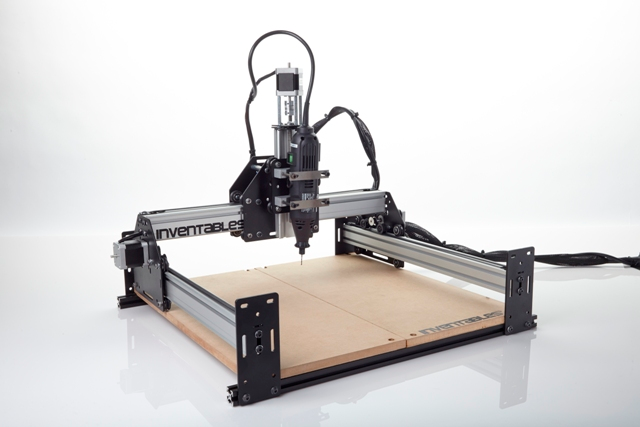
\includegraphics[scale=0.5]{ch-2/image6.png}
	}
	\caption{Трёхкоординатный фрезерный станок, реализованный в рамках открытого проекта \textit{Shapeoko}.}\label{fig:shapeoko}
\end{figure}

На данный момент проект находится на очень ранней стадии развития, поэтому не удалось провести детальный и всесторонний анализ недостатков представляемого проекта. Тем не менее, некоторые из них можно выделить уже сейчас:
\begin{itemize}
	\item Проект ориентирован в основном на трёхкоординатную фрезерную обработку и не позиционируется как модульная универсальная платформа.
	
	\item Управление опять отдается на откуп обычного персонального компьютера, за тем лишь исключением, что вместе пакета EMC2 авторы предлагают собственное программное обеспечение. О создании какой-либо модульной электронной системы управления речи не идет.
	
	\item Также как и в предыдущем проекте отсутствует какая-либо обратная связь по положению рабочего органа.
	
	\item Для передвижения портала использованы два шаговых двигателя, никак механически не синхронизированные между собой.
	
	\item Перемещение портала осуществляется за счёт зубчатых ремней, при этом не предусмотрены датчики обрыва ремня.
	
	\item Линейное перемещение всех координатных осей осуществляется за счет роликовых кареток. Сложность и~большое количество подвижных частей подобного механизма снижает надежность платформы. Также очевидно, что подобное решение может приводить к заклиниванию осей.
	
	\item В качестве основного и единственного на сегодняшний день рабочего органа используется гравер.
\end{itemize}

Последний параметр, выбранный для сравнения "--- \textit{модульная открытая архитектура блока управления} в совокупности с открытым исходным микрокодом электронного оборудования.

По данному параметру был найден единственный проект "--- анонсированный на 2015 год корпорацией Google модульный смартфон Ara. Безусловно, трудно производить сравнение модульной системы управления оборудования с ЧПУ и мобильную платформу для создания телефонов и планшетов, но такая цель и не ставилась.

Выбор был обусловлен уникальностью данного проекта. Подобные идеи звучали из уст представителей многих известных компаний и научных центров и ранее, но первая успешная попытка создать достаточно сложное электронное устройство из отдельных взаимозаменяемых модулей была сделана только сейчас. Очевидно, что это актуальное направление в ближайшее время получит свое развитие, также очевидно, что оно является очень перспективным и требует всестороннего исследования.

В силу своей специфики достоинства и недостатки проекта Ara рассматриваться не будут, вместо этого будет сделан обзор наиболее интересных и концептуальных решений, реализуемых в рамках данного проекта.

На официальном портале проекта корпорация Google заявляет, что разработала так называемый <<телефон-конструктор>> (рисунок~\cref{fig:ara}). Данный конструктор состоит из двух частей: эндоскелета (также часто называемого <<рамой>> и являющегося, по сути, внутренним каркасом) и~набора сменных модулей.

\begin{figure}[ht]
	\centerfloat{
		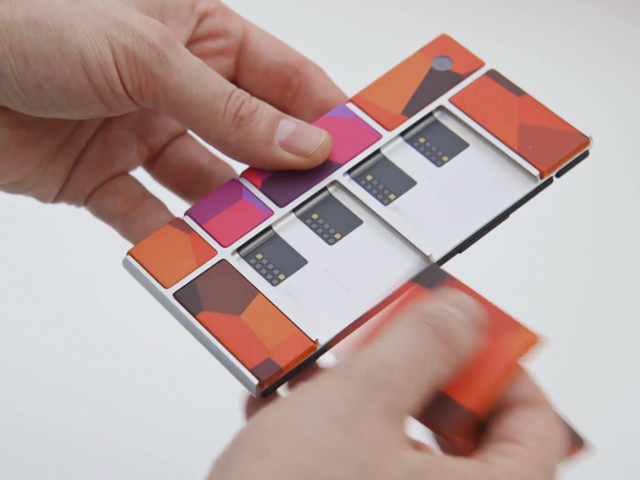
\includegraphics[scale=0.5]{ch-2/image7}
	}
	\caption{Модульный смартфон Ara.}\label{fig:ara}
\end{figure}

К эндоскелету могут быть подключены процессор со всей необходимой электрической <<обвязкой>>, жидкокристаллический дисплей, дополнительные модули оперативной памяти, физическая клавиатура, камера или дополнительный аккумулятор. Владелец телефон сможет сам производить модернизацию своего устройства или заменять поврежденные модули. Какие-то специальные инструменты или наличие каких-то знаний в области микроэлектроники или программирования не требуются.

Также за счет унификации габаритов эндоскелета и проектируемых модулей можно изменять размер аппарата, предполагается возможность создания как небольшого и очень компактного устройства, так и устройства, сравнимого по своим размерам с современными смартфонами и даже устройства больше похожего на интернет-планшет, а не мобильный телефон.

Очевидное достоинство подобного подхода для пользователя "--- возможность подбирать модули в соответствии со своими потребностями и финансовыми возможностями. Специалисты компании Google говорят, что в минимальной комплектации модульный смартфон будет стоить порядка 50 долларов США, а в максимальной "--- до 500.

Платформа позиционируется как открытая, то есть любой сторонний разработчик, использую так называемый MDK (сокр.~от~англ. \textit{Module Developers Kit} "--- набор инструментальных средств разработчика для создания модулей), сможет выпустить свой модуль, совместимый с Ara.

В спецификации говорится, что некоторые модули могут поддерживать так называемую <<горячую замену>>, то есть возможность сменить модуль без отключения питания аппарата. Также оговорен унифицированный способ крепления модулей к эндоскелету "--- крепление будет осуществляться за счет постоянных магнитов.

Каждый модуль может сочетать в себе несколько различных функций, например, можно создать гибридный модуль, являющийся экраном мобильного телефона и дополнительным аккумулятором, компенсирующим затраты энергии на подсветку и отображение информации.

Телефоны Ara будут работать под управлением операционной системы с открытым исходным кодом Android, что подтверждает полную программную и аппаратную открытость рассматриваемого проекта.

\section{Современные тенденции в области стандартизации модульного оборудования}

\subsection{Концепция Module Type Package (MTP)}

На сегодняшний день модульный подход находит свое применение в обрабатывающей промышленности. В частности, наиболее проработанной является концепция NAMUR Module Type Package (MTP), применяемая в областях специальных химических производств, а также в фармацевтической промышленности. Концепция формализована в виде стандарта VDI/VDE/NAMUR 2658. В обрабатывающей промышленности модульные производственные системы играют более важную роль в силу своей повсеместной применимости. Одним из ярких представителей модульного производства в автоматизации производства является стандарт PackML для упаковочных машин. Несмотря на схожие концепции и бизнес-преимущества модульной автоматизации, требования и текущая техническая реализация описания модуля и оркестровки процессов различаются в разных отраслях. Этот факт увеличивает необходимые усилия по внедрению гибридных, то есть межотраслевых приложений. Одним из типичных гибридных приложений является процесс производства химических жидкостей с последующим розливом в бутылки, включая непрерывную часть процесса (например, фактическое производство) и дискретную часть (например, розлив, этикетирование, транспортировку). В работе [grothoff2020mapping] описывается процесс выявления сходств и различий между существующими подходами к модульной автоматизации. В этом документе основное внимание уделяется интерфейсам управления процессами, которые обычно развертываются в самом модуле и доступны через OPC UA. Наряду с существующими стандартами, такими как MTP и PackML, мы также обсуждаем подход к управлению процессами, который был разработан в рамках финансируемых проектов BaSys 4.0 и BaSys 4.2 и проверен на демонстрации. Для получения инженерной информации о модулях BaSys использует модули, такие как сериализация различных файлов или API (например, интерфейсы XML или RESTful с полезной нагрузкой JSON) или инфраструктуру, подходящую для модульного подхода, например серверы обнаружения для обнаружения компонентов и метаданных.

В соответствии со стандартом MTP производственные модули могут быть от разных производителей, так как функциональность модуля описана в независимой от поставщика оборудования [bloch2018state]. Одна часть MTP описывает сервисы, которые реализует модуль. В этих сервисах заключены автоматизация полевых устройств модуля и взаимодействие полевых устройств. Таким образом, функция процесса может быть запущена без необходимости управления отдельными полевыми устройствами. Сервисы являются основным элементом модульных технологических установок, потому что они представляют собой новый уровень в иерархии автоматизации. В дополнении к этому модульная технологическая система содержит человеко-машинный интерфейс блок оркестровки. Блок оркестровки взаимодействует со службами, которые управляют полевыми устройствами в модулях. Прямое влияние на полевые устройства в рабочем автоматическом режиме невозможно, что является самым большим отличием от классических технологических установок. Непрямая адресация полевых устройств с помощью сервисов обеспечивает целостность модуля и защищает ноу-хау поставщика модуля.

Проектирование модульных технологических установок делится на два разных этапа: а) модульное проектирование и б) интеграционное проектирование. На первом этапе поставщик модуля проектирует и реализует модуль, на втором этапе уже в рамках производственного процесса на конкретном предприятии все модули объединяется в единую технологическую установку. Интерфейс между этими двумя "--- это MTP как независимое от производителя описание модуля. На первом этапе проектирования поставщик модуля должен спроектировать сервисы модуля. Следовательно, основные функции процесса в разумных комбинациях должны быть инкапсулированы как сервисы. Следовательно, необходимо учитывать различные аспекты, такие как аспекты проектирования процесса, аспекты устройства и аспекты автоматизации. Поскольку трудно определить, какой способ инкапсуляции и комбинации является разумным, этот вклад сталкивается с инкапсуляцией с точки зрения автоматизации.

\section{Выводы по главе 1}

В рамках диссертационной работы исследуются модели и методы построения модульных систем. Подчеркивается, что проблема эффективности работы модульного оборудования до сих пор не решена из-за серьезных различий в подходах к проектированию подобного оборудования и его применения в приборостроительном производстве, что пока не позволяет выполнять эффективное моделирование и переконфигурирования модульных производственных системы. На данный момент не существует эффективных методов и моделей проектирования и разработки модульного оборудования, более того практически отсутствуют единые стандарты проектирования модульного оборудования. Для создания эффективной методики проектирования и использования модульного оборудования необходимо проводить глубокий анализ условий предприятий, работающих в новых и высокоинтеллектуальных отраслях производства, а также в условиях постоянной смены номенклатуры производимых высокотехнологичного оборудования.

\FloatBarrier
